% 1907 words

\subsection{Key Questions}
what was the scope and how was it defined \\
what filters were used \\
what were the walking and cycling speeds used \\
what were the travel times calculated \\
what was the directness of travel on different networks \\
what is the distribution of travel times in the different networks \\
what lsoas changed the most and least across networks \\
how did removing road types affect the number of lsoa centers connected? \\
how long did the calculations take? \\
Did removing directionality from the networks have a significant effect? \\
Did removing directionality mediate the effect of removing primary and trunk streets? \\


%%%%%%%%%%%%%%%%%%%%%%%%%%%%%%
\subsection{Scope}


Scope was defined to capture the largest computationally feasible network with a simple set of rules. 

The first rule was to restrict the network to ``Inner London''. This has the advantage of a formal designation by the GLA for each borough (\cite{innerlondon}). The second rule was to restrict the scope to the area north of the River Thames. This has two advantages. First it further refines the study area to a higher density segment of the city with a higher portion of journeys to work done by bicycle. Second, it removes the need for a trip to cross the river via a bridge. Including bridges in the analysis would have made drawing conclusions more difficult as the ability to cross the river would have been a deciding factor in the possibility of a journey and a key determinant of the journey's distance, requiring a cyclist to go far out of their way to use one of only a dozen bridges potentially available. 

Table \ref{table:commute_data} contains some data about journeys to work in the scope of the study area. The area defined captures 18\% of the population, 16.8\% of the working adults, and 25\% of the jobs in the city. 8.2\% of the journey's to work are contained in this area. Additionally, rates of cycling are higher in inner London than in the periphery as seen in the 5\% rate of cycling between locations within the area compared to the 2.4\% London average. Finally, the area contains 25\% of the traffic incidents where a cyclist was killed or seriously injured between 1989 and 2004 (\cite{cyclistksi}). 
 
\begin{table}[]
\centering
\begin{tabular}{lcccl}
 Mode Share Within Scope & All Modes & Bicycle & \% by bicycle &  \\
 \hline
 Origin in scope &  981,354 & 46,832 & 4.8\% &  \\
 Destination in scope & 1,454,606 & 48,461 & 3.3\% &  \\
 Both in scope & 479,882 & 24,843 & 5.2\% & \\
 All journeys & 5,852,298 & 140,180 & 2.4\% \\ 
\end{tabular}
\caption{Journeys to work by location and type}
\label{table:commute_data}
\end{table}

%%%%%%%%%%%%%%%%%%%%%%%%%%%%%%
\subsection{Defining Networks}

There are three possible ways to construct a set of ways and nodes from OSM. These are; a positive filter; a negative filter; and selecting by relation. A positive filter specifies tags that an way or node must have to be included. A negative filter includes all ways and nodes without the tags specified. A relation is the OSM term for a collection of ways and nodes that belong to a set identified by an OSM contributor. 

OSM relations in London identified as being cycle routes are mapped in Figure \ref{fig:bicycle_relation}. The query for selecting this set can be found in the Appendix table \ref{table:osm_tags}. It is clear that this is an extensive set of geometries. Clearly though the density of that network is fairly low and for almost any trip a user would need to venture beyond the relation geometries. Further, many of the ways included in the cycling relations are in fact no different from other streets. As seen in Figure \ref{fig:brandon} a picture of Brandon Way. This has no safety improvements for cyclists, it has been observed that speeds can far exceed the 20 mph limit. Thus, the cycle relations on their own are insufficient for building representative networks. 

good example of the difficulty of building a good network representation is Castle Baynard St. It connects the Central London part of cycle superhighway 3 with the East London section that continues out to Limehouse. This is a tunnel that serves as a bike path and as a driveway of sorts to an underground car park. A network built from the relation[route=bicycle] set of ways and nodes would include this but despite being quite and low traffic the street has no dedicated cycle infrastructure, therefore tagged as ``highway = unclassified''. 

"to measure miles of designated bike facilities can be misleading. Some designated bicycling facilities involve LTS values that most people will not tolerate" (\cite{furth2016network}).

Add paragraph comparing bicycle relation to primary+trunk network. 

Some of this content is also in the Data OSM section...

In the case of the relation, the Camden Hackney Quietway was examined in person. Figure \ref{fig:brandon} shows an image of Brandon rd, a part of the Quietway. This way is tagged ``highway=unclassified'' and connects to Agar Grove, tagged ``highway = tertiary''. The unclassified marker indicates that the street is less important than a tertiary street but is neither residential or a service road. As can been seen in the image, Brandon Rd. has no actual cycle infrastructure. There is a tag noting the max speed is 20 mph. Data collected for 20 mph streets found that as many as 80\% of drivers exceeded these limits. 
% https://www.thesun.co.uk/news/7253694/20-mph-zones-cause-more-deaths/

In other cases, OSM underestimates the quality of cycling infrastructure. For instance the intersection of Mile end Road and Cambridge Health Road in the borough of tower hamlets is a high traffic intersection both for automobiles and for cyclists. It is an integral part of the Stratford to Aldgate cycle super highway. This intersection has been reworked to be safer for cyclists. In OpenStreetMap though, it is labeled a "trunk" highway, due to its high traffic nature. It is way 7058092014. There is also a tag cycleway:left=lane indicating that there is a cyclelane on the left side of the street. (\cite{osm})


\begin{figure}
\centering
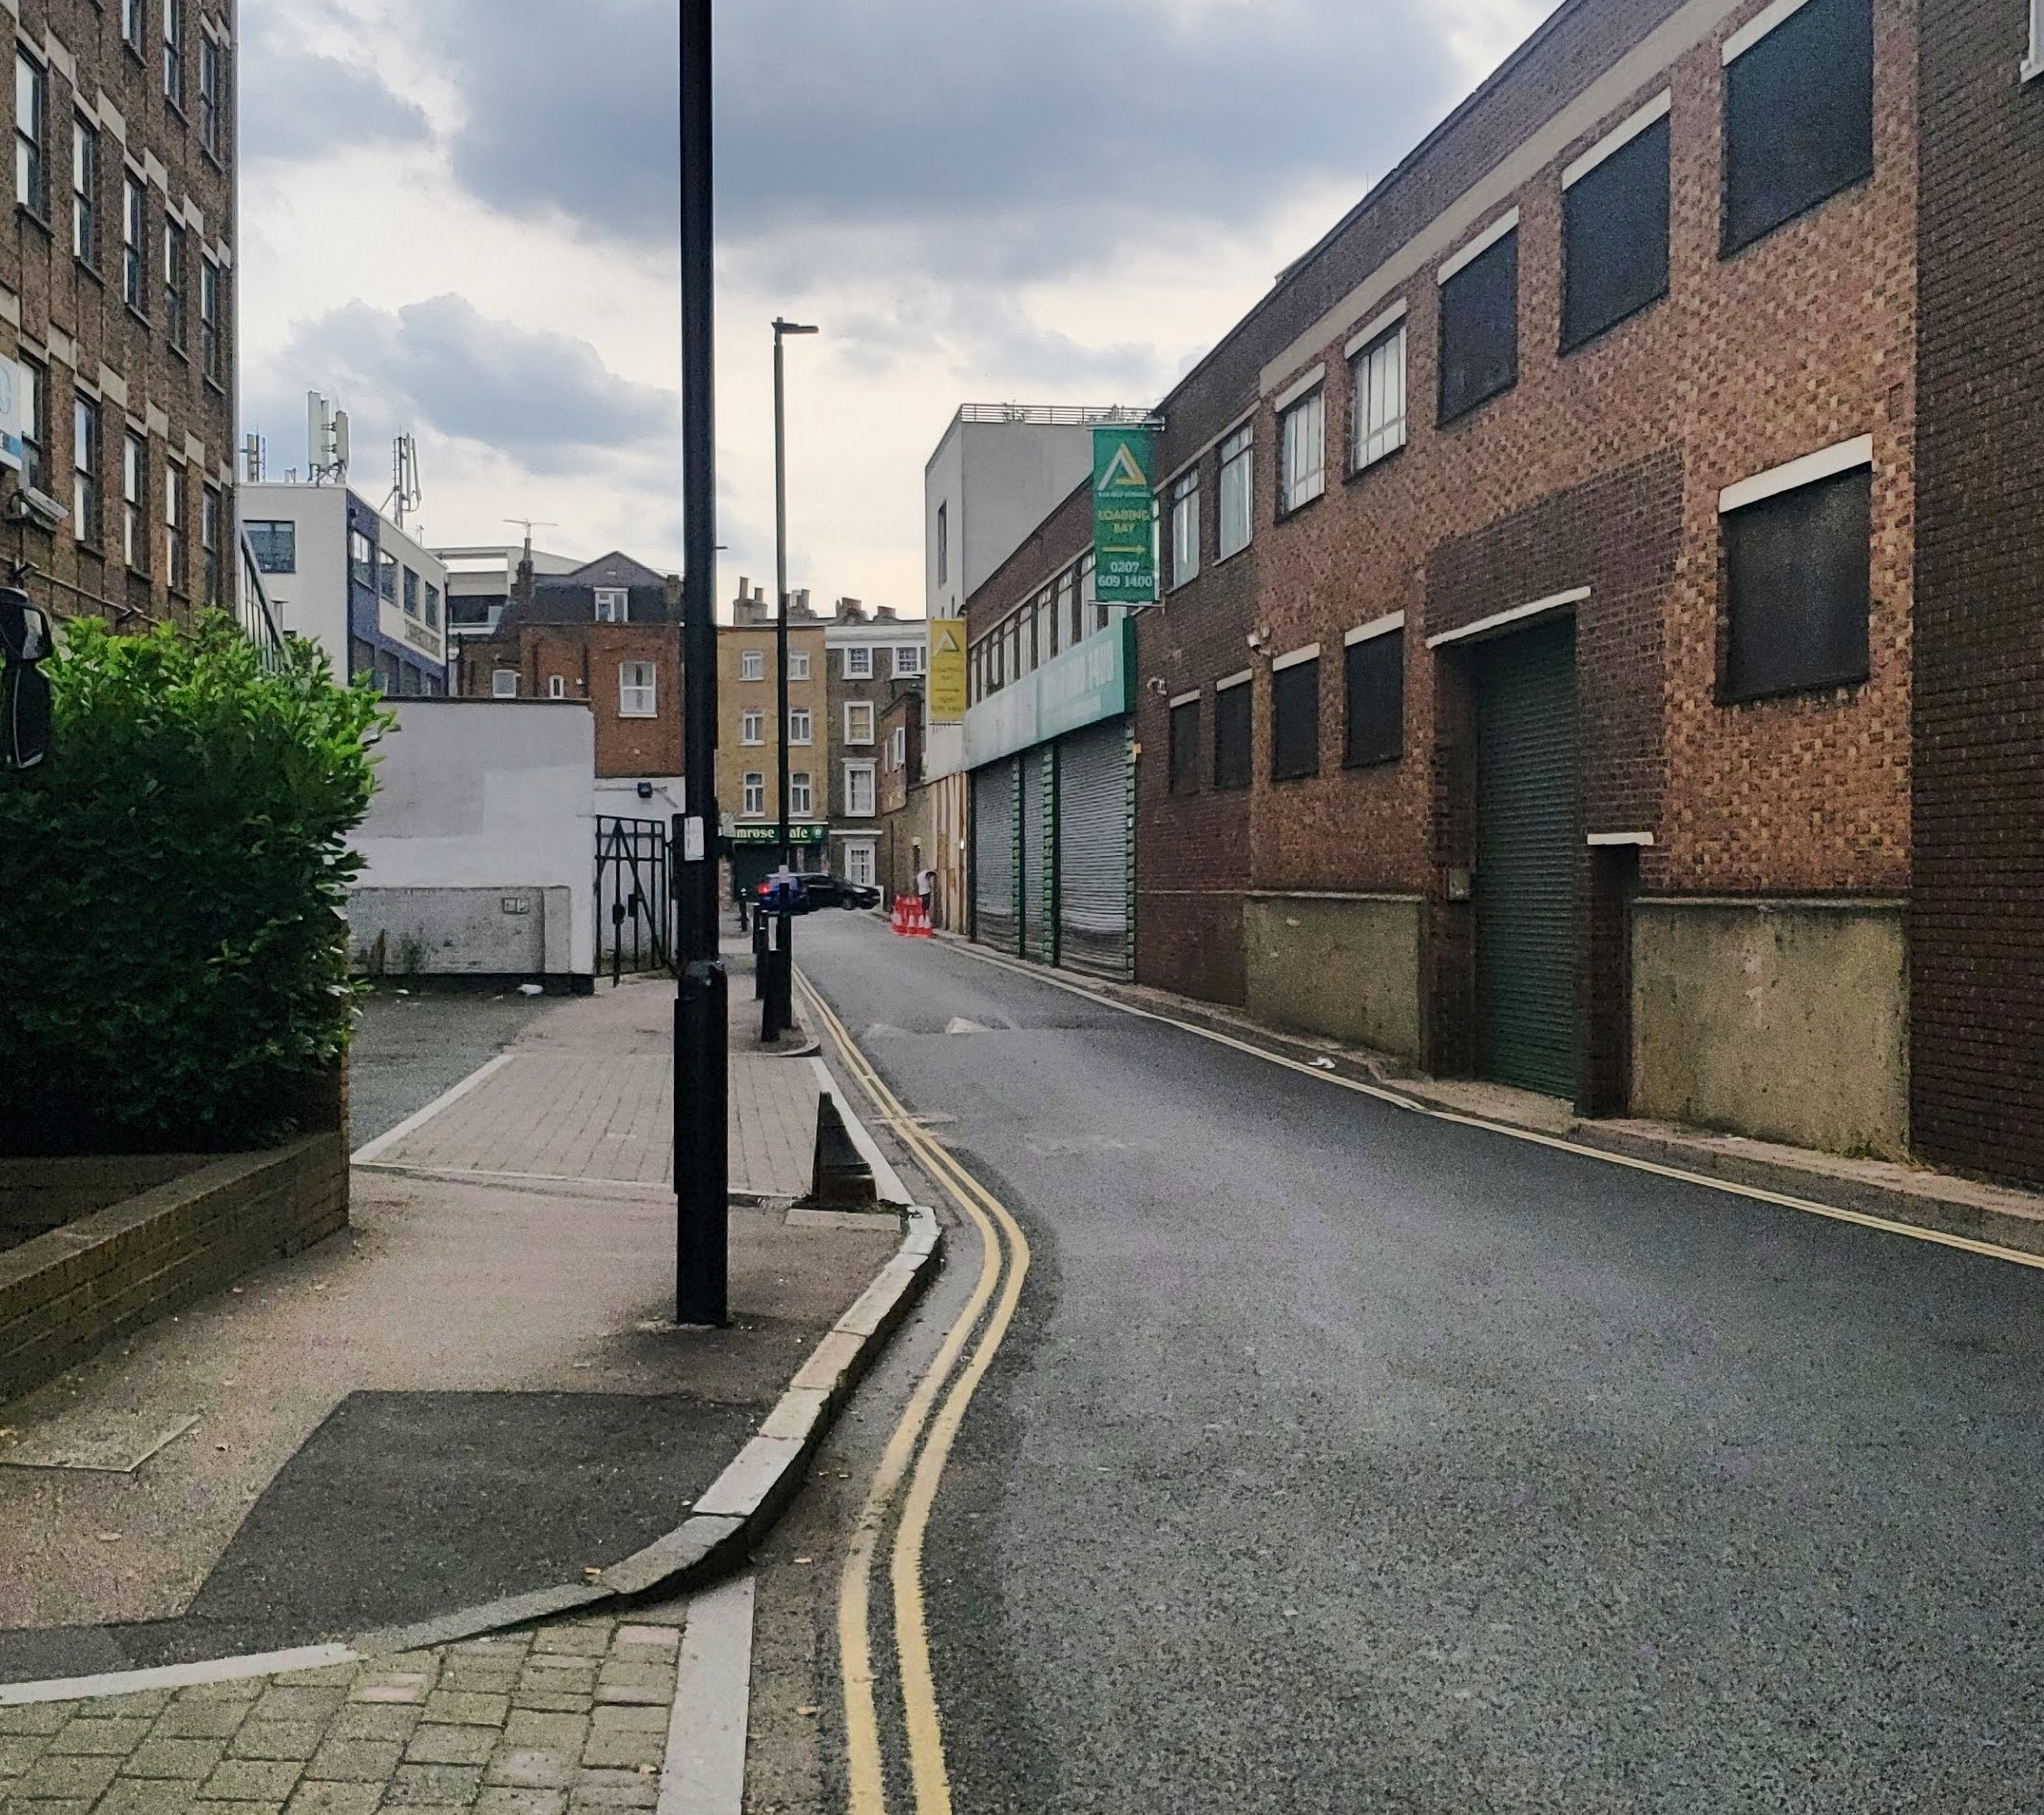
\includegraphics[width=0.6\textwidth]{brandon_rd_cropped}
\caption{Camden Hackney Quietway}
\label{fig:brandon}
\end{figure}

\begin{figure}
\centering
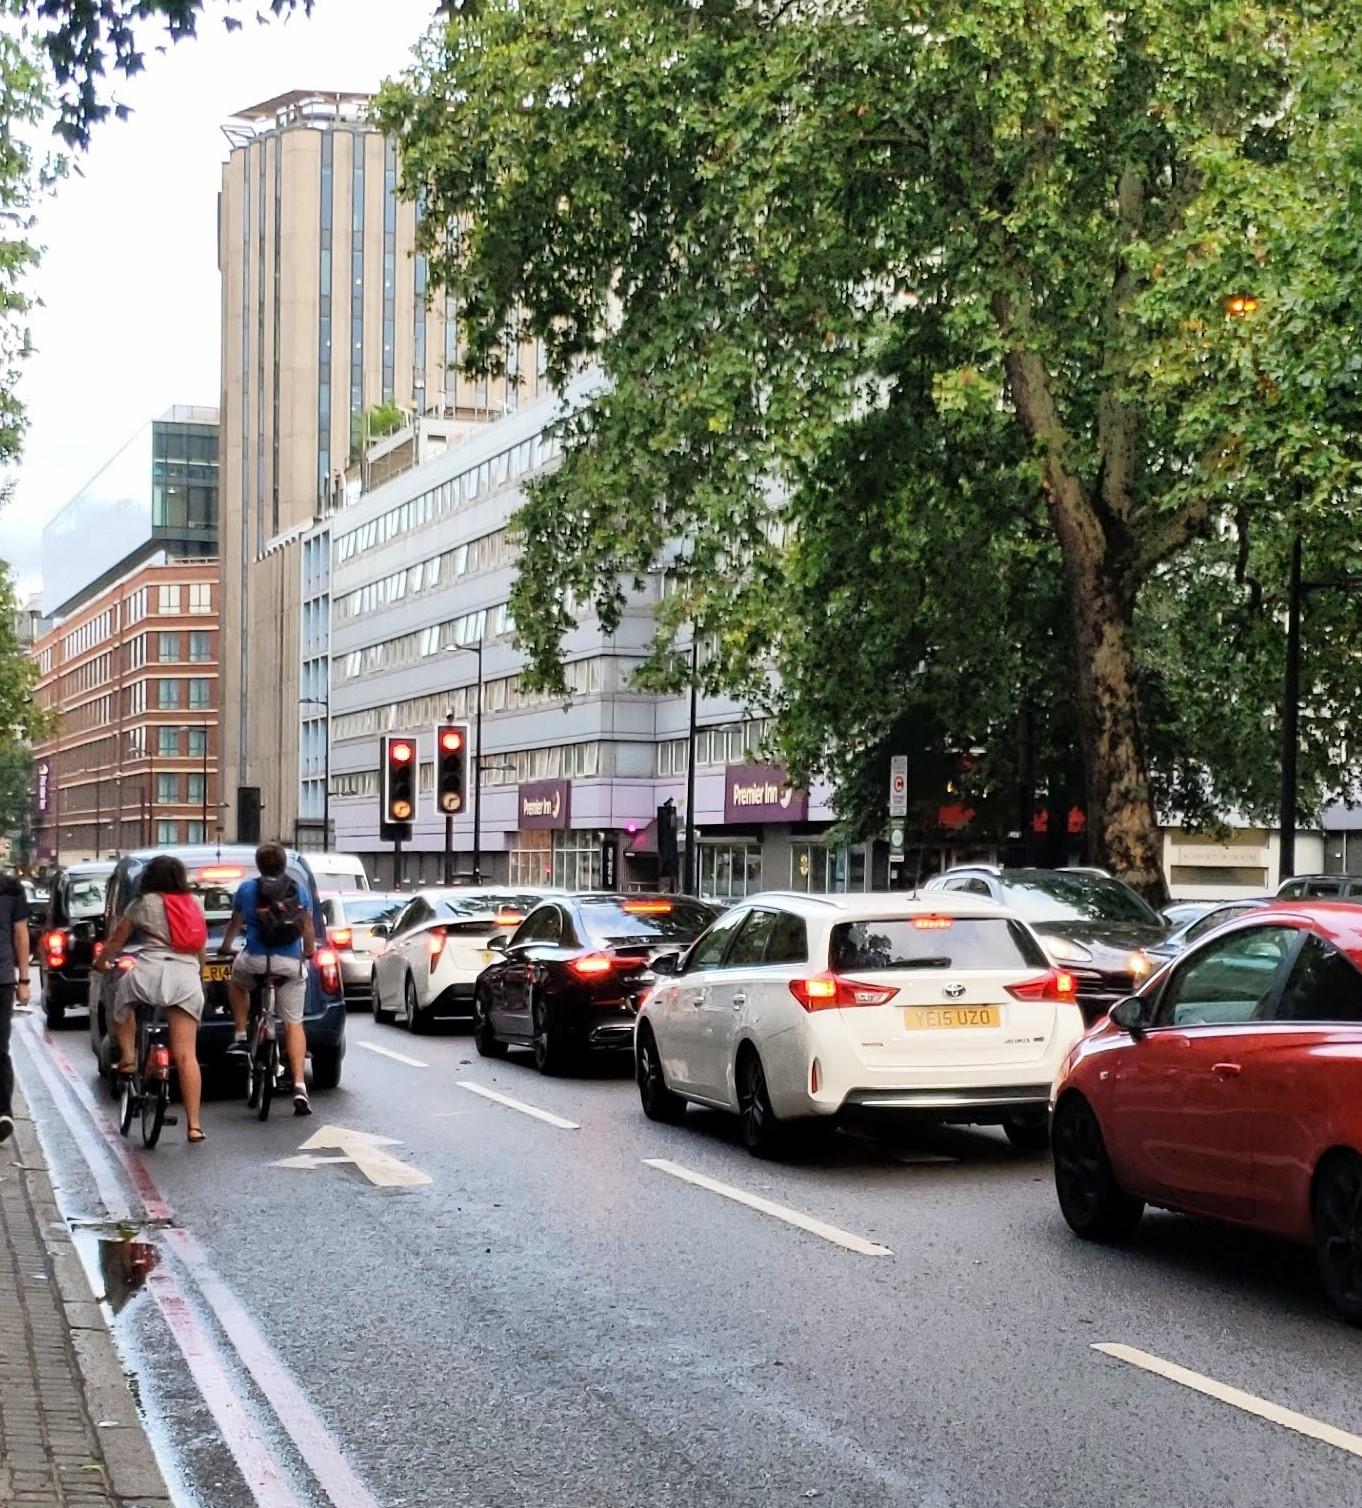
\includegraphics[width=0.6\textwidth]{euston_rd_cropped}
\caption{Euston Road}
\label{fig:euston}
\end{figure}

\begin{figure}
  \centering
%  \includegraphics[width=0.5\linewidth]{}
  \caption{Castle Baynard St}
  \label{fig:baynard}
\end{figure}

\begin{figure}
\centering
\includegraphics[width=0.85\linewidth]{relations}
\caption{Relations identified as bicycle related.}
\label{fig:bicycle_relation}
\end{figure}

A positive filter was explored as a way to include exactly the edges and nodes that met a given level of stress for cycling. This method was challenged by the fact that a single road segment not tagged accurately would disconnect a network part. Further, there was not a method found to work correctly for selecting roads with any one of many tag values.  Table \ref{table:osm_tags} details all of the possible tags related to cycling that were found in the London OSM data.  In the Overpass Turbo application, this could be accomplished by using multiple subqueries as detailed in the Overpass Turbo Cycling network query listed in the Appendix. In OSMnx this multiple query statement structure was not an option. Thus a method for building full and accurate networks of OSM geometries using a positive filter was not found. 




\begin{figure}
\centering
\includegraphics[width=0.85\linewidth]{primary_trunk}
\caption{Highways tagged primary or trunk}
\label{fig:primary_trunk}
\end{figure}

The negative filter, implemented as a modification of the filters built into OSMnx version 0.11dev was the most successful. The first filter included all ways and nodes not explicitly tagged with values indicating that cycling was not allowed. Row XXXX of Appendix \ref{table:filters}. The second filter was the same as the first but excluded streets tagged as primary and trunk. These are the two tags used for the highest priority street types as seen in Table \ref{table:osm_tags} describing standard tags for the ``highway'' key in OSM. These streets are visualized in Figure ~\ref{fig:primary_trunk} The third filter restricted secondary streets in addition to the restrictions of the second. The fourth filter restricted tertiary streets leaving only living and residential streets in a addition to non-motor vehicle ways like canal paths and segregated cycle lanes. The final filter, 5, restricted all edges where a cyclist might interact with motor vehicles. Samples of these filters are displayed in Figures ~\ref{fig:sub1} through ~\ref{fig:sub4}

\begin{figure}
  \centering
  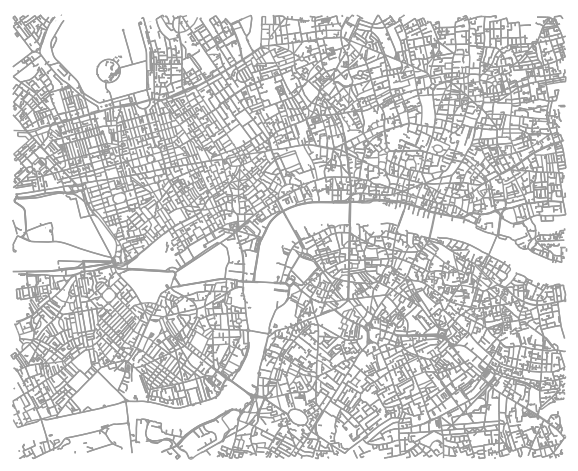
\includegraphics[width=0.5\linewidth]{bbox_bike_1_filter_cropped}
  \caption{Filter 1: most confident cyclists}
  \label{fig:sub1}
\end{figure}

\begin{figure}
  \centering
  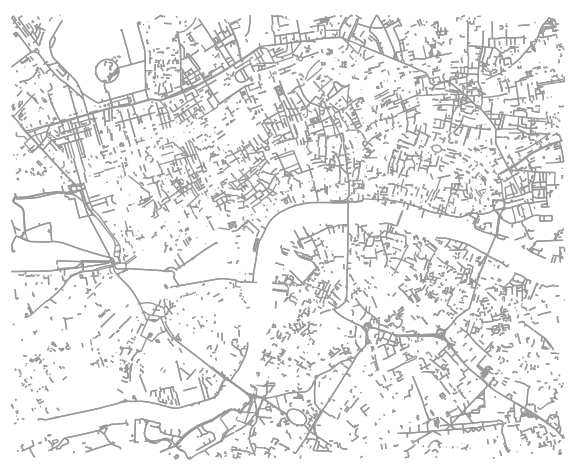
\includegraphics[width=0.5\linewidth]{bbox_bike_5_filter_cropped}
  \caption{Filter 5: no interaction with cars }
  \label{fig:sub2}
\end{figure}

Lastly, two more networks were specified. These were networks 1 and 2, all streets and all streets but primary and trunk, with the directionality of the streets removed. These networks would be used to test the effect of direction restrictions on travel times and whether removing direction restrictions for cyclists could successfully replace the need to use some more busy and dangerous streets. 

\begin{figure}
  \centering
  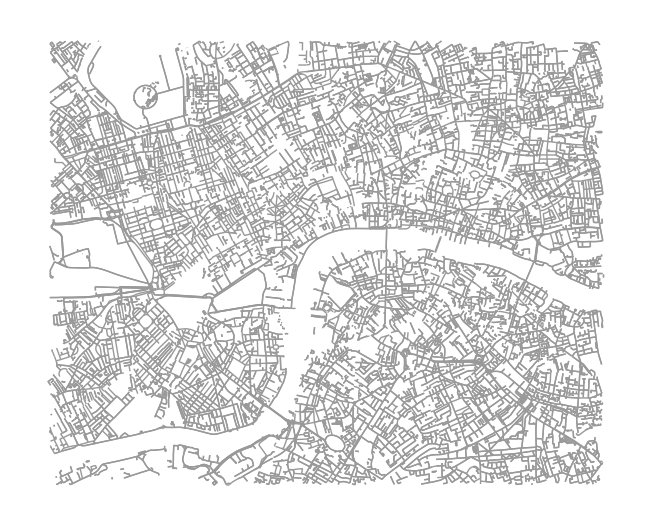
\includegraphics[width=0.5\linewidth]{bbox_bike_2_filter_cropped}
  \caption{Filter 3: all but primary and trunk streets}
  \label{fig:sub3}
\end{figure}



\begin{figure}
  \centering
  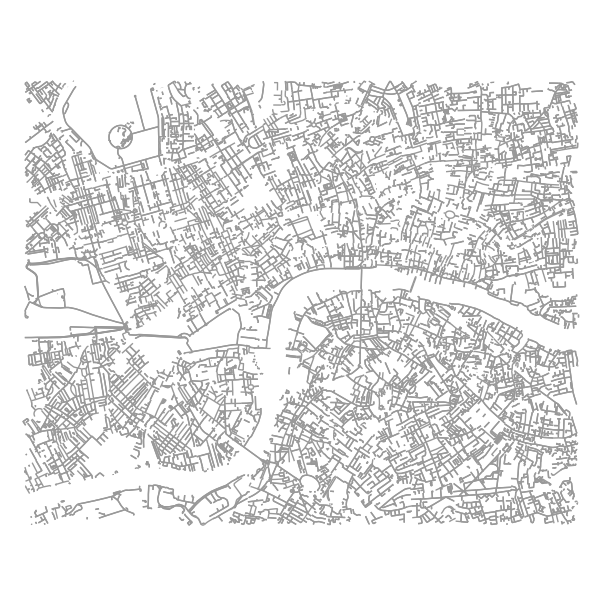
\includegraphics[width=0.5\linewidth]{bbox_bike_4_filter_cropped}
  \caption{Filter 4: only residential and living streets}
  \label{fig:sub4}
\end{figure}

The weakness of the negative filter was the inability to include streets tagged as multiple types. Negative filter 2 excluded any highway tagged primary regardless of whether it was also tagged with cycleway or cycleway:left=lane. Thus the negative filters also do not fully reflect the reality of the London street network for a cyclist. However, it was the best method for testing the importance of street types and the effect of directionality on travel times. 

%%%%%%%%%%%%%%%%%%%%%%%%%%%%%%
%\subsubsection{Network Characteristics}
%
%chart of largest connected component of network as edge types are included.  Figure ~\ref{fig:connected_component}. Table ~\ref{table:network_stats}.

%\begin{figure}
%\centering
%\caption{largest component of network type}
%\label{fig:connected_component}
%\end{figure}

%\begin{table}
%\centering
%\caption{table of network statistics}
%\label{table:network_stats}
%\end{table}
 
 %%%%%%%%%%%%%%%%%%%%%%%%%%%%%%
\subsubsection{Quant Network}

The QUANT dataset has 23,377,225 pairs of origins and destinations. The subset matching the scope of this investigation has 799,236 pairs. That subset has 200,041 missing distances. 

To complete the missing distances, the quant travel times were built into a networkx multidigraph. There was an edge for each node pair that represented the walking time between the nodes, calculated as the straightline distance between the nodes divided by the google walking speed 3 mph converted to 4.83 kph and converted to  0.0805 kilometers per minute giving a number of minutes walking time between the nodes that was in the same units as the number of minutes public transit time between the nodes. 

Then for each pair of nodes missing a transit time, the shortest path on the graph was calculated. Thus each travel time can be a combination of walking and riding public transit between nodes. 

%%%%%%%%%%%%%%%%%%%%%%%%%%%%%%
\subsection{Origins and Destinations}

One origin/destination node was selected for each LSOA. The node was selected as the node from the set of nodes across all network definitions that was closest to the centroid of the LSOA polygon. This is essentially a sampling technique. While individual nodes may give strange results due to the specifics of their locations, it is expected that the average results for 894 nodes that yield 798,342 origin destination pairs will be a sufficiently large sample that individual idiosyncracies balance out. 

As seen in Figure~\ref{fig:dist_diffs} the distribution of the differences between the distance between centroids and the distance between actual nodes is well balanced. 

\begin{figure}
\centering
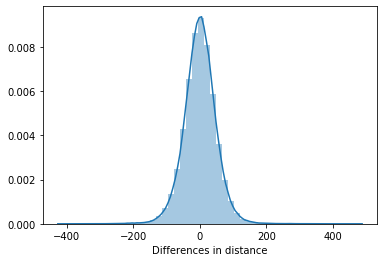
\includegraphics[width=0.5\linewidth]{node_centroid_dist_diff}
\caption{Distribution of distances between nodes minus distances between centroids}
\label{fig:dist_diffs}
\end{figure}

\begin{figure}
\centering
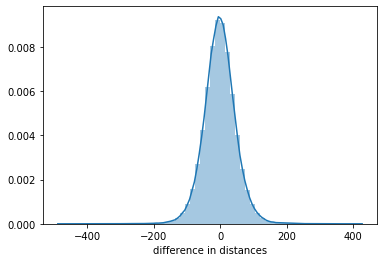
\includegraphics[width=0.5\linewidth]{quant_node_dist_diff}
\caption{Distribution of distances between cycle network nodes minus distances between QUANT nodes}
\label{fig:quant_dist_diffs}
\end{figure}

Node 5816785884, closest to the centroid of LSOA XXXXXX is found at the entrance to a garage at the end of a one way street. Thus every other node in the network is inaccessible on the directed versions of the network. The edge leading to this node is tagged ``service'' so perhaps service streets should have been excluded as they are frequently dead ends. 

Because urban density increases as one approached the center of a city, there could be a slight bias towards node distances being lower than centroid distances. This is because there is a higher probability that the closest node will be on the central side of the centroid than the outside. This was investigated and as seen in Figure ~\ref{fig:diff_dist}, the distribution of differences in straightline distances was well balanced around 0. The same consideration was checked for the differences between distances for cycling nodes and the distances between the nodes used in the QUANT calculations. Seen in Figure ~\ref{fig:quant_dist_diffs}, that distribution was also well balanced around 0. 

%\begin{figure}
%\centering
%\caption{\% of connected pairs by network}
%\label{fig:connected_pairs}
%\end{figure}

%%%%%%%%%%%%%%%%%%%%%%%%%%%%%%
\subsection{Travel Times}

Travel times were converted from distances using a walking speed of 3 mph and a cycling speed of 8 mph based on data taken from google maps estimates for journeys as seen in that table. These were converted to kilometers per minutes, waking: $0.0805$ and biking $0.215$. 

\begin{table}
\centering
\caption{Google Maps travel speeds}
\label{table:travel_speeds}
\end{table}

As seen table XXXXX travel times for bike network 2, without trunk or primary highways, are substantially longer than travel times for bike network 1. This indicates that the effect of removing these edges is not just to disconnect the network but also requires a network user to take a less direct route, straying further from the straight line between origin and destination. 

The difference between directed and undirected distances is also notable. 

the standard deviation 

the min is unchanged, while the max 

Travel times by bicycle for aggressive cyclists are XXXXX compared to the QUANT travel times by public transport. 

Transit times are consistently lower than cycling times. However, transit times are from hub to hub, so there is in most cases, an additional walking time to get from the transit hub to the actual destination that would be less of a factor for a journey by bicycle. 

The connectedness estimated may understate the true connectedness. This is seen in that unconnected node pairs in almost every case have one node that is unconnected from all other nodes. Thus there are not local islands of connectivity, there are nodes being disconnected from the network due to the removal of a single edge. 

The network doesn't really fracture. Where connectivity goes down, it is usually an individual node becoming disconnected from all others, not a sub group being separated of. MOst nodes not connected to another node, were not connected to any other nodes. 


\begin{table}
\centering
\begin{tabular}{@{}lllll@{}}
\toprule
networks & u\_1   & d\_1  & u\_2            & d\_2          \\ \midrule
         &        &       & \multicolumn{2}{l}{$\Delta$ time (mins)}  \\
u\_1     & x      &  0.79 & 8.16            & 14.46         \\
d\_1     & 0      & x     & 7.38            & 13.68         \\
u\_2     & 36.9   & 36.9  & x               & 6.30          \\
d\_2     & 47.8   & 47.8  & 4.7             & x             \\
         & \multicolumn{3}{l}{$\Delta$ \% connected} &               \\ \bottomrule
\end{tabular}
\caption{Changes between networks, \% connected and directness}
\label{table:change between nets}
\end{table}

There's got to be a significant difference between the distances for the different networks right?


\begin{table}[]
%\centering
\begin{tabular}{lrrrrrrrrr}
\toprule
network                  & u\_1    & d\_1    & u\_2  & d\_2  & quant & quant+ & d\_3 & d\_4 & d\_5 \\ \hline
                         &         &         &       &       &       &        &      &      &      \\
largest component edges  &         &         &       &       &  -    & -      &      &      &      \\
\% pairs connected       & 100     & 100     &  63.1 & 58.2  & 74.9  & 100    & 21.9 & 1.4  & 0.03 \\
average directness *     & 1.20    & 1.23    & 1.53  & 1.80  & -     & -      & -    & -    & -    \\
min travel time*         & 0.4     & 0.4     & 0.4   & 0.4   & 0.1   & -      & -    & -    & -    \\
mean travel time*        & 33.0    & 33.8    & 41.1  & 47.4  & 22.6  & -      & -    & -    & -    \\
max travel time*         & 88.8    & 91.2    & 114.0 & 124.0 & 51.9  & -      & -    & -    & -    \\
travel time std. dev*    & 16.8    & 17.1    & 20.4  & 23.6  & 8.6   & -      & -    & -    & -   \\ \bottomrule
\end{tabular}
\caption{Network routing statistics \\ $*$ includes only pairs connected by all networks.}
\label{table:travel_time_stats}
\end{table}

\begin{table}
\centering
\caption{travel time statistics}
\label{table:travel_time_stats}
\end{table}

%%%%%%%%%%%%%%%%%%%%%%%%%%%%%%
\subsubsection{Maps}

lsoa's colored by travel times difference between cycling and quant. 

\begin{figure}
\centering
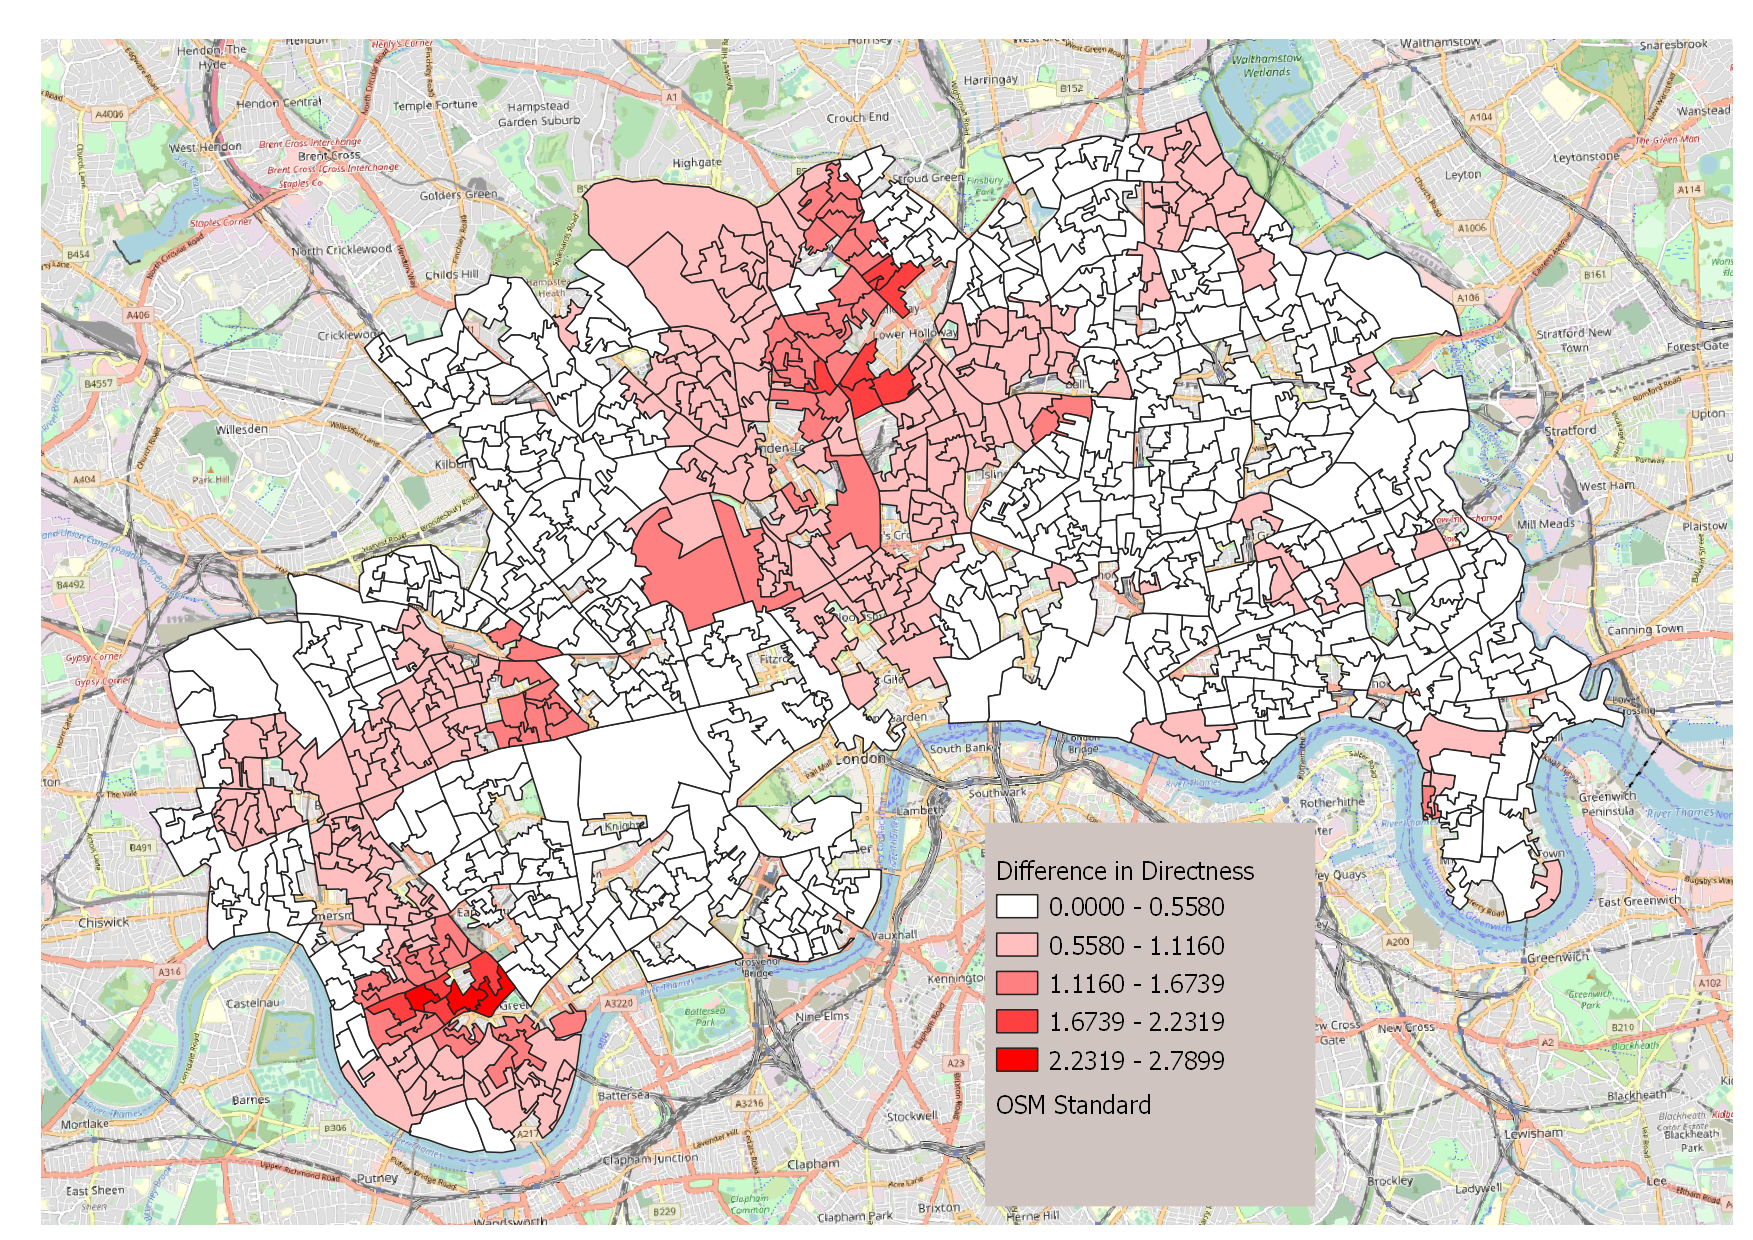
\includegraphics[width=0.85\linewidth]{d_1_d_2_directness}
\caption{Difference in directness D1 and D2}
\label{fig:d1_d2_directness}
\end{figure}


lsoa's colored by change in directness 

\begin{figure}
\centering
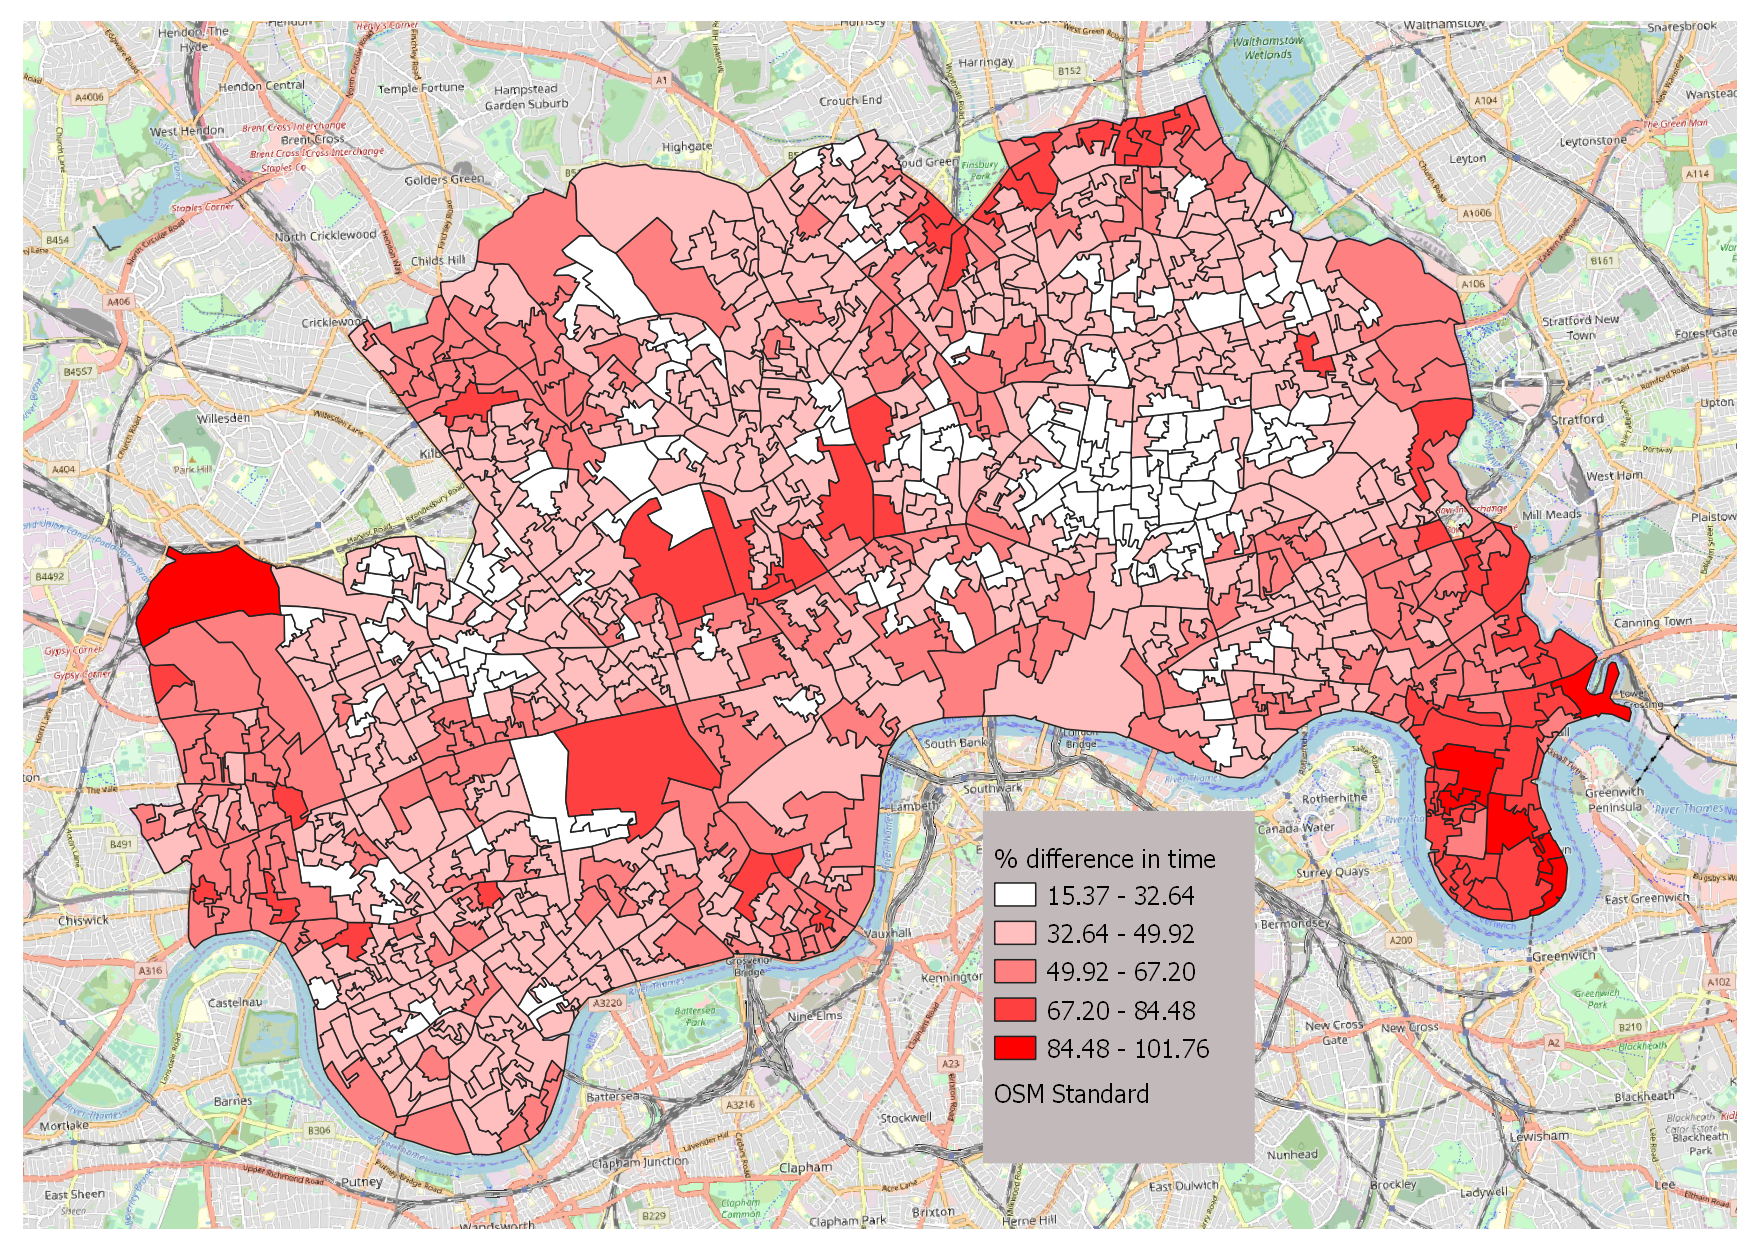
\includegraphics[width=0.85\linewidth]{quant_plus_d1_time_diff_perc}
\caption{\% ddifferent in travel time, QUANT+ and D1}
\label{fig:quant_d1_time}
\end{figure}

%\begin{figure}
%\centering
%\caption{LSOA's colored by directness of routes to other lsoas}
%\label{fig:lsoa_directness}
%\end{figure}

%%%%%%%%%%%%%%%%%%%%%%%%%%%%%%
\subsubsection{distributions of travel times}

insert histograms of directness and travel times
\begin{figure}
\centering
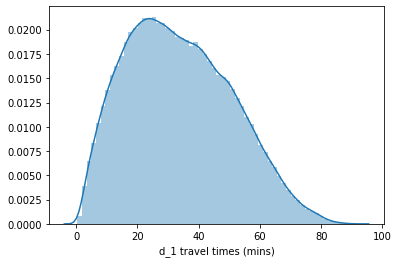
\includegraphics[width=0.85\linewidth]{d_1_travel_times_dist}
\caption{Distribution of travel times for D1}
\label{fig:d1_distrib}
\end{figure}

\begin{figure}
\centering
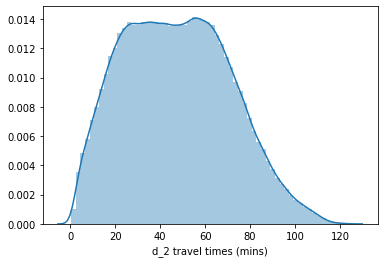
\includegraphics[width=0.85\linewidth]{d_2_travel_times}
\caption{Distribution of travel times for D1}
\label{fig:d2_distrib}
\end{figure}

\begin{figure}
\centering
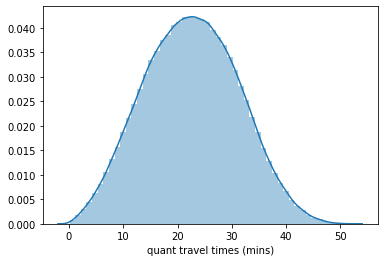
\includegraphics[width=0.85\linewidth]{quant_travel_times_dist}
\caption{Distribution of QUANT public transit travel times}
\label{fig:quant_distrib}
\end{figure}


%%%%%%%%%%%%%%%%%%%%%%%%%%%%%%
\subsection{Changes in Routing}

Seen in Figure \ref{fig:routing_1} and \ref{fig:routing_2} compare longest path for directed network 2 to the path between those nodes in directed network 1. 

Compare longest path for directed network 1 to undirected network 1. 

compare o/d pair with largest increase in distance between directed 1 and directed 2 to the distance in undirected 2. 

Is allowing travel in any direction on side roads a good replacement for primary and trunk routes?


\begin{figure}
\centering
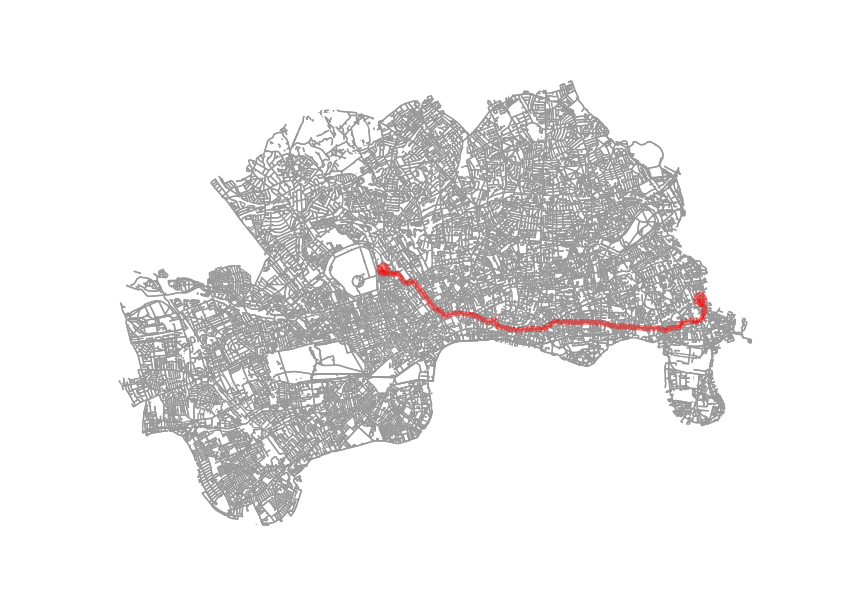
\includegraphics[width=0.85\linewidth]{route_diff_d1_ex9}
\caption{Example of routing on directed network 1}
\label{fig:routing_1}
\end{figure}

\begin{figure}
\centering
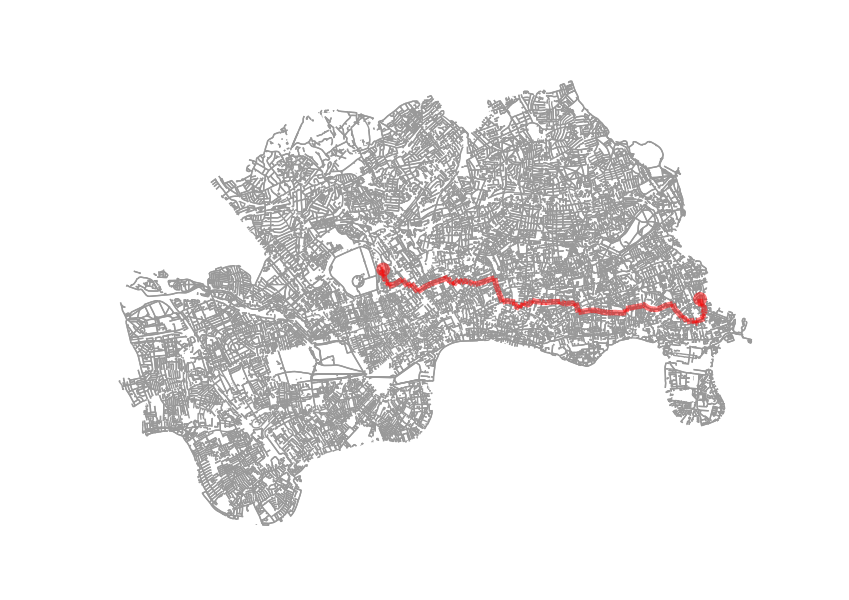
\includegraphics[width=0.85\linewidth]{route_diff_d2_ex9}
\caption{Example of routing on directed network 2}
\label{fig:routing_2}
\end{figure}

%%%%%%%%%%%%%%%%%%%%%%%%%%%%%%
\subsection{Accessibility}

connectivity ratio.

 

simple \% of trips possible

\% of trips possible with time restriction. 

in qgis, color lsoa's by travel time to central lsoa. 

in QGIS color lsoa's by travel time from lsoa with highest average distance. 

in QGIS color lsoa's by  average directness, distance divided by straightline distance. 

Plot a few paths in osmnx to look at low directness. 





%%%%%%%%%%%%%%%%%%%%%%%%%%%%%%
\subsection{Notes about computation}

runtimes for the distances between nodes were long. computations were done on an intel i74700HQ processor with the database contained on the internal Solid State Drive. 

Runtimes increased with the number of connected origin destination pairs, since unconnected pairs  did not require the calculation of a shortest path. Thus bike 1 travel times took longer than bike level 2. Additionally, the undirected network calculations took substantially longer than the directed networks because there were sugnificantly more route possibilities with more edges available at each node. 

Table \ref{table:net_calc_times} contains calculation times by network type. 

% table for computation times across algorithm types

% table for computation times across network types
%\begin{table}[]
%\centering
%\begin{tabular}{lllll}
%network  & 1 & 1 undirected & 2  & 2 undirected   \\
%time     & 24:00   & 72:00??  & 9:03  & 36:00        \\        
%\end{tabular}
%\caption{Computation Times}
%\label{table:1}
%\end{table}

\begin{table}[]
\centering
\begin{tabular}{@{}l|llll@{}}
network     & 1           & 1 undirected & 2    & 2 undirected \\ \hline
time(hours) & 24 & 72  & 9 & 36
\end{tabular}
\caption{Calculation times for routes}
\label{table:net_calc_times}
\end{table}

%\begin{table}
%\centering
%\caption{Computation times using different algorithms}
%\label{table:comp_times_algo}
%\end{table}


text